\documentclass[11pt]{article}

\usepackage[margin = 1 in]{geometry}
\usepackage[pdftex]{graphicx}
\graphicspath{{images/}}
\usepackage{subfigure}
\usepackage{booktabs}
\usepackage{multirow}
\usepackage[table]{xcolor}
\usepackage{array}
%\usepackage{amsmath}
\usepackage{booktabs}
\usepackage{multirow}
\usepackage{amsmath}
\usepackage{url}

\hyphenation{op-tical net-works semi-conduc-tor re-co-mmen-ded}


\title{Project Group 3}
\author{ Johnathan Salamanca, Mario Cer\'{o}n, \\
Carol Martinez, Javier Cocunubo, Jairo Nino, Alvaro Munoz
 }
\date{\today}

\begin{document}
\maketitle

%\begin{abstract}

%In this document \ldots
%\end{abstract}


\section{Introduction}
\label{sec:Intro}
Introduction section of final report written.
This should clearly state the context of your team?s application and the problem you set out to solve, as well as your justification for why it is an important problem.



\section{Multiple Problem Versions}
\label{sec:app}
%All versions should naturally build on top of each other
%? V1 should be pretty easy and reasonable
%? The last version can be moonshot - the idea is that you must implement
%for V1 first, then V2, etc. so as to guarantee some sort of finished build by
%the end of Week 10. If you can get to V2, V3, etc. by the end, great, if not,
%at the very least you have something done that you can present)
%Business Problem. Your main task is to explore the data and identify patterns of crime in Chicago, and come up with strategies to efficiently deploy your workforce to fight crime.

\textbf{Version 1}\\

The Municipal Capacities-Adjusted Disaster Risk Index is an innovative indicator for policymakers to make informed decisions about how to better preserve citizens\' well-being in the presence of real and potential threats. However, to be actionable, information needs not only to be available but efficiently delivered to communities, as a mean of protecting citizen\'s rights, foster economic growth, and make government officials accountable. 

As per its current state, official risk management information lacks a delivery system that enables local communities to improve their risk awareness and disaster coping capabilities in different scenarios marked for global phenomena such as extreme temperatures and changing weather patterns.
For instance, it is not apparent how similar events have impacted communities with different risk and vulnerability profiles, and there is no relevant information to assess the performance of risk management activities.  

%\begin{itemize}
%\item{There is no information available online wit the Disaster Risks panorama in Colombia}
%\item{The information available online about Disaster Risks in Colombia corresponds to Excel files, and to some reports created by the government with insights of the Disaster Risks panorama in Colombia. However, the information is not published in such a way that anyone can use to get easy-to-see information about the current risk state of a specific area. }
%\end{itemize}


\subsection{Question}

Based on the previously presented information different questions have arisen.

\begin{enumerate}


\item{In 2012, the National System of Risk Management was created in Colombia. Based on the available datasets is it possible to analyze and find patterns that show (\textbf{V3}),
\begin{itemize}
\item how does the risk map of Colombia changed after the creation of this system?
\end{itemize}
}


\item{There is a disproportionate impact of similar events among Colombia's municipalities, given by disparities in available infrastructure and first response resources  (\textbf{V2}).}


\item{Is it possible to analyze a specific event (disaster) and show how does the same event  affects different zones of the country? Based on that, we can analyze (\textbf{V1}):
\begin{itemize}
\item Are there factors that make some zones more vulnerable than others?
\item How does the specific infrastructure affects the impact of the specific event?
\end{itemize}
}
\end{enumerate}

%\subsection{Question}


\section{Datasets sourced }
\label{sec:app}

The main dataset used in the project is from the Colombia Risk of Disaster Management Unit (Unidad de Gesti\'{o}n de Riesgos y Desastres) UNGRD \cite{datasetUNGRD}. The dataset contains information about  the risk management associated with natural phenomena, socio-natural, technologic, and human-based non-intentional incidents reported in Colombia in the last 10 years (38626 records). Some of the fields found in the dataset are: Date, Department, Municipality, Event Name, Code, Dead, Wounded, Disappeared, Affected People, Affected Families, Affected Houses, among others.

The team will also use a dataset from the National Administrative Department for Statistics DANE. It is a time series between 1985 to 2020 and contains information, per department code about \cite{DANE} .

Both datasets contain ``DIVIPOLA'' codes, which is the codification of the Politica-Administrative Division of Colombia (Codification of the departments, ). Figure \ref{fig:divipola} describes the meaning of the code. The first two numbers correspond to the department, followed by the Municipality Code and the Populated Center [\cite{divipola}].


\begin{figure}[!ht]
        \center{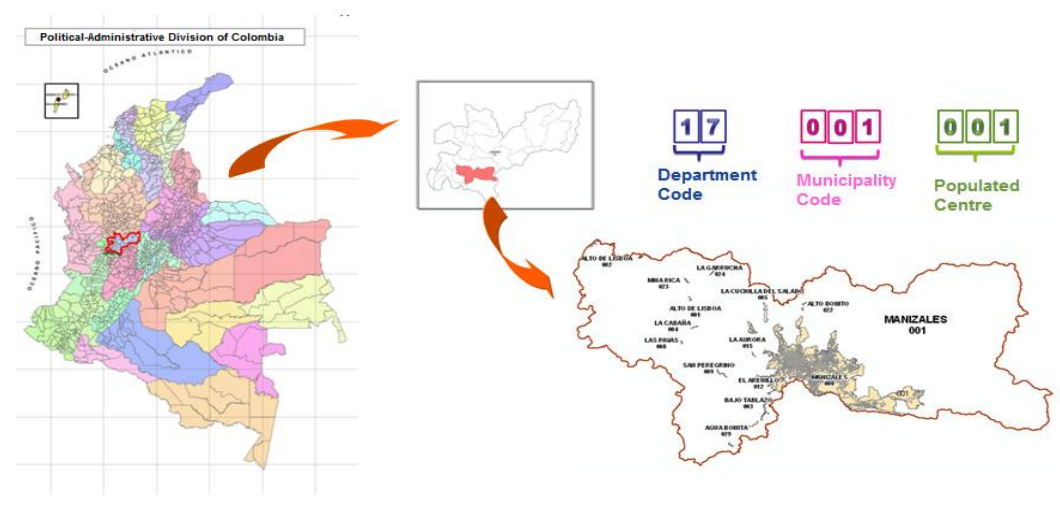
\includegraphics[width=0.6\textwidth]
        {divipolaExplanation}}
        \caption{Explanation of ``DIVIPOLA'' code. The codes provide information of the Politica-Administrative Division of Colombia. Image taken from \cite{divipola}}
        \label{fig:divipola}
      \end{figure}


%Table \ref{tabDataset} summarizes the information of the datasets.
%
%\begin{table}[h]
%\begin{center}
%\label{tabDataset}
%\begin{tabular}{|c|c|c|c|c|}
%\hline
%\textbf{Data Name} & \textbf{Description} & \textbf{Type} & \textbf{Number} & \textbf{Database}   \\
%\hline
% Event name: & type of disaster (flooding,XX)& categorical &S &  UNGRD\\
% Date: & incident date & numerical &XXX &  UNGRD/DANE  \\
% Code: &disaster ID & numerical &XXX &  UNGRD/DANE  \\
% Municipality Code: & Divipola code & numerical &XXX &  UNGRD/DANE  \\
% Dead: & Deads per incident & numerical &XXX &  UNGRD  \\
% Wounded: & Wound per incident & numerical &XXX &  UNGRD  \\
% Disappeared: & Disappeared per incident & numerical &XXX &  UNGRD  \\
%  Affected: & Affected people & numerical &XXX &  UNGRD  \\
%   Affected families: & Affected people & numerical &XXX &  UNGRD  \\
%\hline
%\end{tabular}
% \caption{Summary of the main information available to develop the project.}
%\end{center}
%\end{table}
%



%  (data of ):
%http://portal.gestiondelriesgo.gov.co/Paginas/Consolidado-Atencion-de-Emergencias.aspx
%We plan to cross data from the previous dataset with data from the DANE, IDEAM
%We may require datasets to extract data of:
%Hospitals available in the area
%Schools
%Emergency services available.
%Demographic data



%Santos talks about Colombia Progress on Risk Management https://www.unisdr.org/archive/58870

%? ?El Ni�o? and particularly the La Ni�a 2010-2011, which generated a national emergency situation never before seen in the country, affecting nearly 765 municipalities in Colombia, ?. After these phenomena, the government decided to improve the gathering information systems (info taken from
%https://library.wmo.int/doc_num.php?explnum_id=4759 )


\section{Project scoping plan/proposal written}
\label{sec:app}

\subsection{Project scope}

\begin{itemize}
\item The Government Officials (at all levels) are our main stakeholders
\item Boundaries of the project:
\begin{itemize}
\item We do not offer forecasts or modeling/ infer data.
\item We only show metrics of impact of disasters at municipal level (not pin point to specific disaster event)
\item We do not offer recommendations, only do support to decision making process for the stakeholders.
\end{itemize}
\item Risks
\begin{itemize}
\item Data quality issues in the datasets 
\item The available data might be not enough to solve the proposed problem.
\end{itemize}
\end{itemize}


\subsection{Project plan}

%\textbf{Problem}: The Municipal Capacities’-Adjusted Disaster Risk Index is an innovative indicator for policymakers to make informed decisions about how to better preserve citizens’ well-being in the presence of real and potential threats.
%However, to be actionable, information needs not only to be available but efficiently delivered to communities. As a means of protecting citizen’s rights, foster economic growth, and make government officials accountable.
%As per its current state, official risk management information lacks a delivery system that enables local communities to improve their risk awareness and disaster coping capabilities in different scenarios marked for global phenomena such as extreme temperatures and changing weather patterns.
%For instance, it is not apparent how similar events have impacted communities with different risk and vulnerability profiles, relevant information to assess the performance of risk management activities.

 %Impact is defined in terms of: Inhabitants affected/Thousand Inhabitants, percentage of households affected, Deceased/ Thousand Inhabitants.\\

\begin{itemize}
\item \textbf{Expected Deliverable}:\\
To cope with the challenges stated before, our approach includes a dynamic map of Colombia delivering:

\begin{enumerate}
\item The impact metric (or metrics) at the municipal level for a given category of events. Ability to display complementary metrics of interest for specific locations (utilities, healthcare facilities, first-responder facilities, etc).
\item Considering the established association between extreme temperatures and the frequency of hydro-meteorological events, a projected extreme-temperature indicator for the 100 most vulnerable municipalities with 3 data points: Indicator value at Time 0 (1998), Time 1 (2018) and Time 3 (projected 2040)
\item The indicator corresponds to the extreme temperature projection made by Climate Impact Lab for the number of days a year that register temperatures above 32 degrees Celsius.
\end{enumerate}




\item \textbf{How do we get there?}:

\begin{itemize}
\item Get datasets, clean, wrangled, and analyze them.
\item Data modeling
\item Load the data in the cloud (RDS on AWS) and the instance (EC2) for hosting the back and front ends. Install and review the environment.
\item Make the back end: review databases, environment and set the code for running in the cloud
\item Make the front end : Interactive Colombian Map in Dash and tested on AWS.
\item Make the final presentation
\item Make the final report
\end{itemize}

\end{itemize}

\section{Application Overview}
\label{sec:appOver}


\subsection{Users}
Any person, Government officials, or someone in the private sector who wants to read and understand the basic risk profile of their region and make decisions with that information.

\subsection{Architecture}

Figure \ref{fig:archi} shows the architecture of the proposed solution including the elements of the application at component level and its connections at high level (see deployment diagram). Additionally, it shows the application elements used for the Front and Back End. The figure also shows the names of the technologies used hosted on AWS cloud, i.e.: (Python, dash and libraries).   

The following is the list AWS components used in the project: 
\begin{enumerate}
\item The machine who host the solution (Elastic Compute Cloud - EC2). 
\item The Database  (Relational Database Service -RDS).
\item The storage for the datasets and GeoJson files for Colombia on the service  (Simple Storage Service - S3) to save these files.
\item The Security group for these services talks with each other and have access from the internet as well.
\item The remote DNS (Domain Name Service) to have a friendly URL for the application on the Apache Web server.
\item A remote code repository (hosted by github). It is used for hosting the source code and documentation. 

\end{enumerate}


\begin{figure}%
\centering
\subfigure[Deployment diagram]{%
\label{fig:first}%
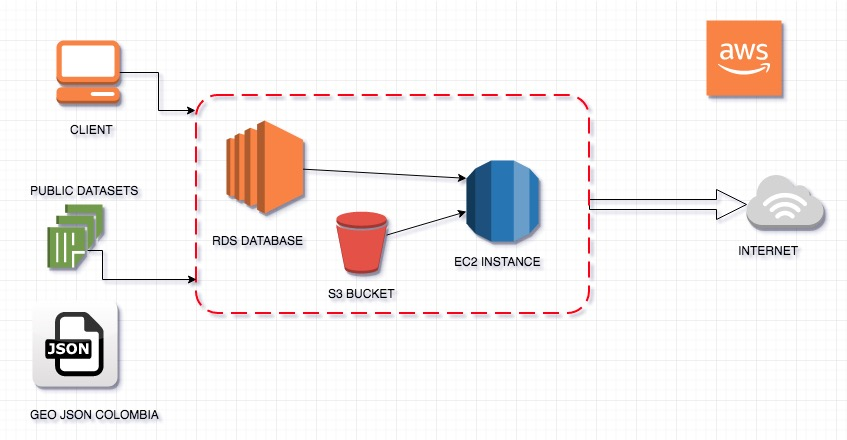
\includegraphics[height=3in, width=4.5in]{../../../aws_diagrams/AWS_Deployment_Diagram_project_group_03}}%
\qquad
\subfigure[Component diagram]{%
\label{fig:second}%
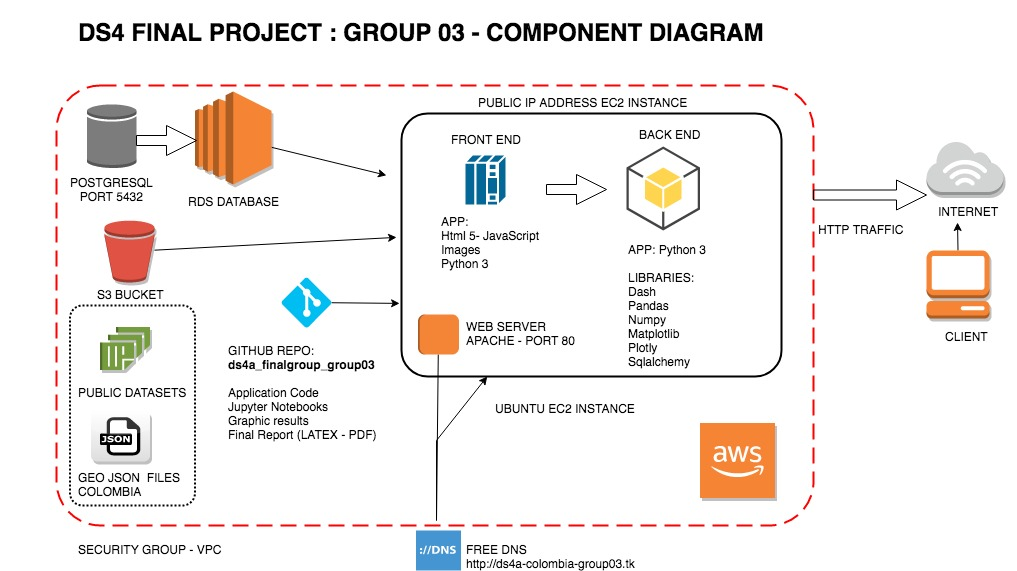
\includegraphics[height=4in, width=6in]{../../../aws_diagrams/AWS_Component_Diagram_project_group_03}}%
\caption{Project architecture.}
\label{fig:archi}%
\end{figure}





\subsection{Front End Design}

The following is the link of the web-page created for the project. \\
 \url{http://ds4a-colombia-group03.tk/}
%\item \href{https://marioceron-case-51.s3.amazonaws.com/final_project/front_end/index.html}{http://ds4a-colombia-group03.tk/} 

In general terms, the proposed information system will provide a dynamic map of Colombia with:

\begin{enumerate}
\item Impact variables such as Deaths, People and Houses affected.
\item A map (Main View) that will show the index adjusted by capacity ( \'Indice Ajustado por Capacidades). By default, the map starts with the country view with political division (departamento).
\item A timeline slider will facilitate the visualization of the index using time intervals. 
\item Considering the established association between extreme temperatures and the frequency of hydro-meteorological events, a projected extreme-temperature indicator for the 100 most vulnerable municipalities with 3 data points: Indicator value at Time 0 (1998), Time 1 (2018) and Time 3 (projected 2040). The indicator corresponds to the extreme temperature projection made by Climate Impact Lab for the number of days a year that register temperatures above 32 degrees Celsius.

\item The option of showing political divisions views (vista de departamento). The user can select the small political subdivision (municipio) and the graphics on the right side of the dashboard screen are updated.
\end{enumerate}




\begin{figure}%
\centering
\subfigure[Presentation page]{%
\label{fig:first}%
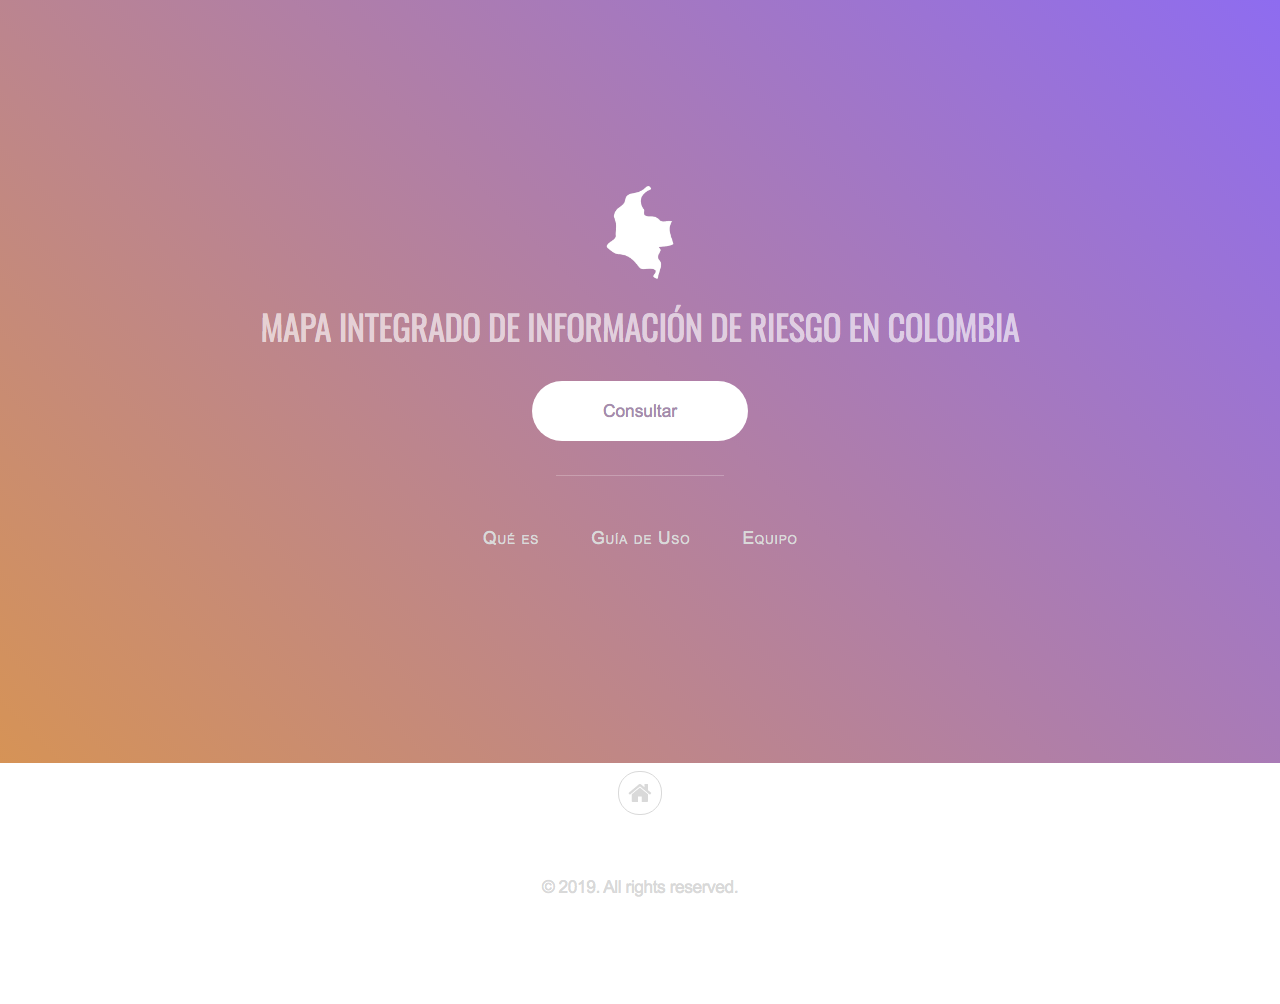
\includegraphics[height=4in, width=6in]{01_Home_ds4a-colombia-group03-tk.png}}%
\qquad
\subfigure[Main page]{%
\label{fig:second}%
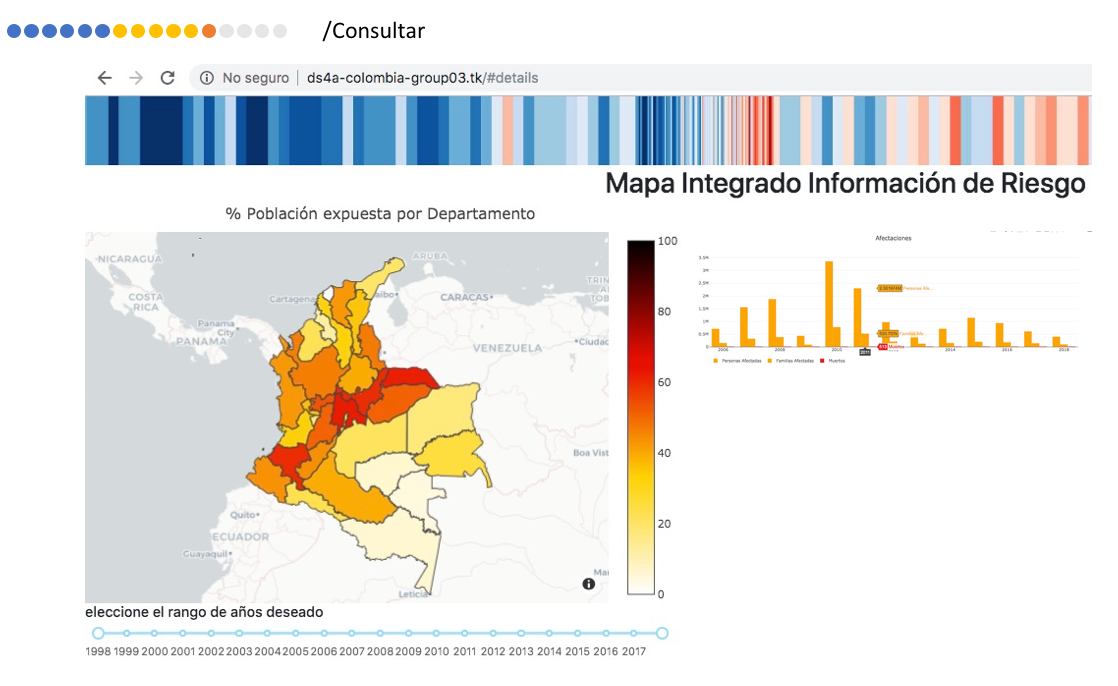
\includegraphics[height=4in, width=6in]{02_Home_mapa.png}}%
%\subfigure[]{%
%\label{fig:second}%
%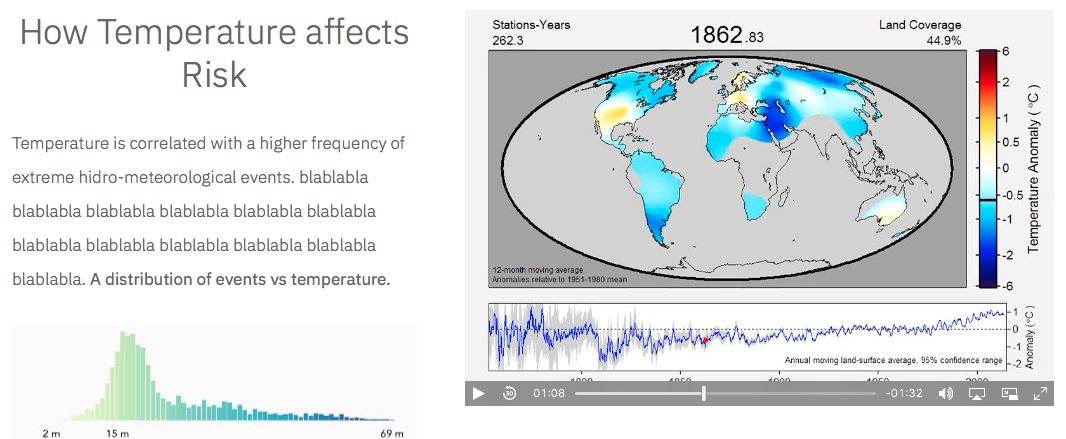
\includegraphics[height=2in, width=3in]{riesgo6}}%
\caption{Front End: Integrated Map of Risk Information in Colombia. The main page (Figure \ref{fig:first}) will show the map of Colombia with the Risk Index, and will offer interactive options to get detail information of selected Municipalities, risk index and a projected temperature indicator.}
\label{fig:muckup}%
\end{figure}


%\section{Technical Information}
\label{sec:Tech}

\subsection{AWS-hosted database}

Figure \ref{fig:er_model} shows the entity relationship model of the project. The information contained in the model is:

\begin{enumerate}

\item Disasters : information of disasters of Colombia from 1998 to 2017, with the following fields: date,  Colombian political division, number of disasters, death, injuries, missing people, families, houses, public and education services infrastructures and some economical  information. (table disasters)
\item Events: name and category of the event (table eventos)
 
\item Political division of Colombia (divipola): ID of division, subdivision and name of both (divipola table)

\item Population estimates: relates population by period, age groups, political division, id, and gender

\item Weather estimates:  weather information from 1990 to 2018 (minimal temperatures, maximal temperatures, precipitations) (tables: historico\_cond\_metereologicas, load\_mintemp, load\_maxtemp, load\_precipitaciones)	


\item Load tables: temporal tables for loading disasters, political division, population (tables: load\_disasters, load\_divipola, load\_populations)

\item Views: wv\_disasters (summary table for disasters). 

\end{enumerate}

The SQL script for the creation of the database on AWS can be download from this link: \\ \url{https://marioceron-case-51.s3.amazonaws.com/final_project/Script_Desastres_DB.sql}{}

Full backup Database: \\ 
\url{https://marioceron-case-51.s3.amazonaws.com/final_project/Script_Desastres_DB_full.sql}{}


 
\begin{figure}[!htb]
\center{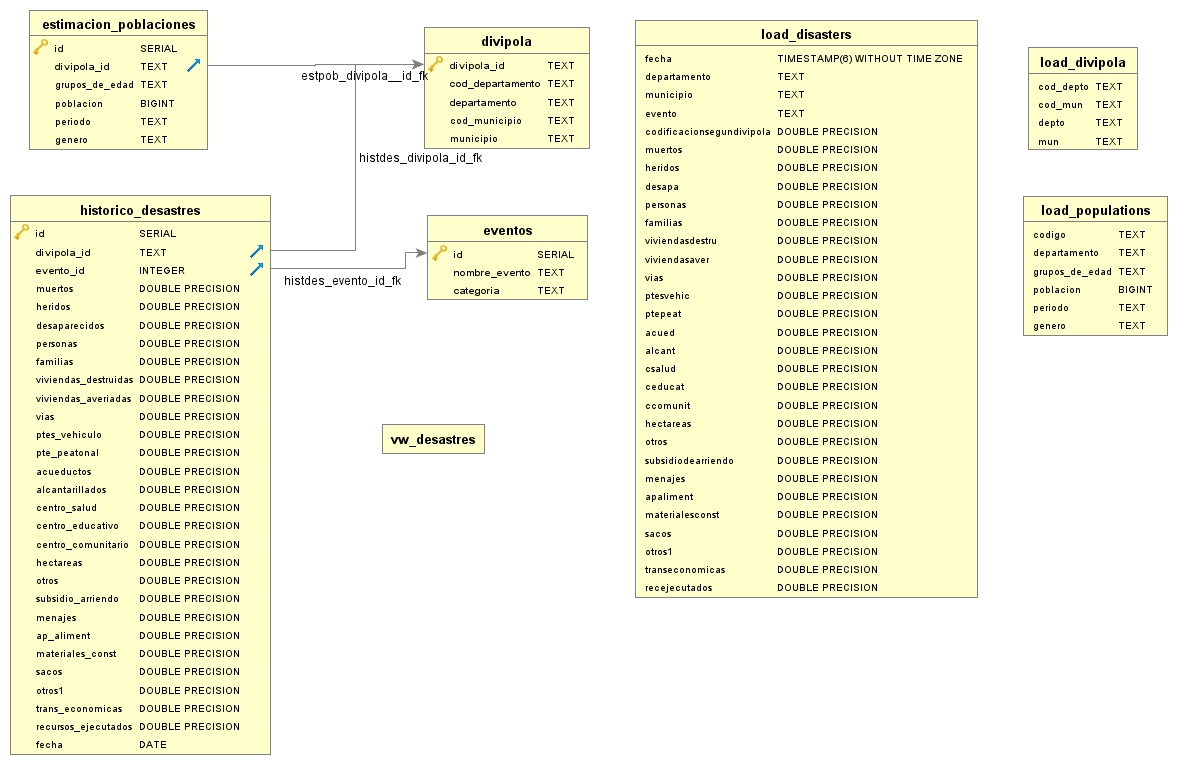
\includegraphics[width=0.95\textwidth]
{Project_Group03_ERModel}}
\caption{Entity relationship model.}
\label{fig:er_model}
\end{figure}

Figure \ref{fig:awsConnection} shows the database uploaded to AWS.

\begin{figure}[!htb]
\center{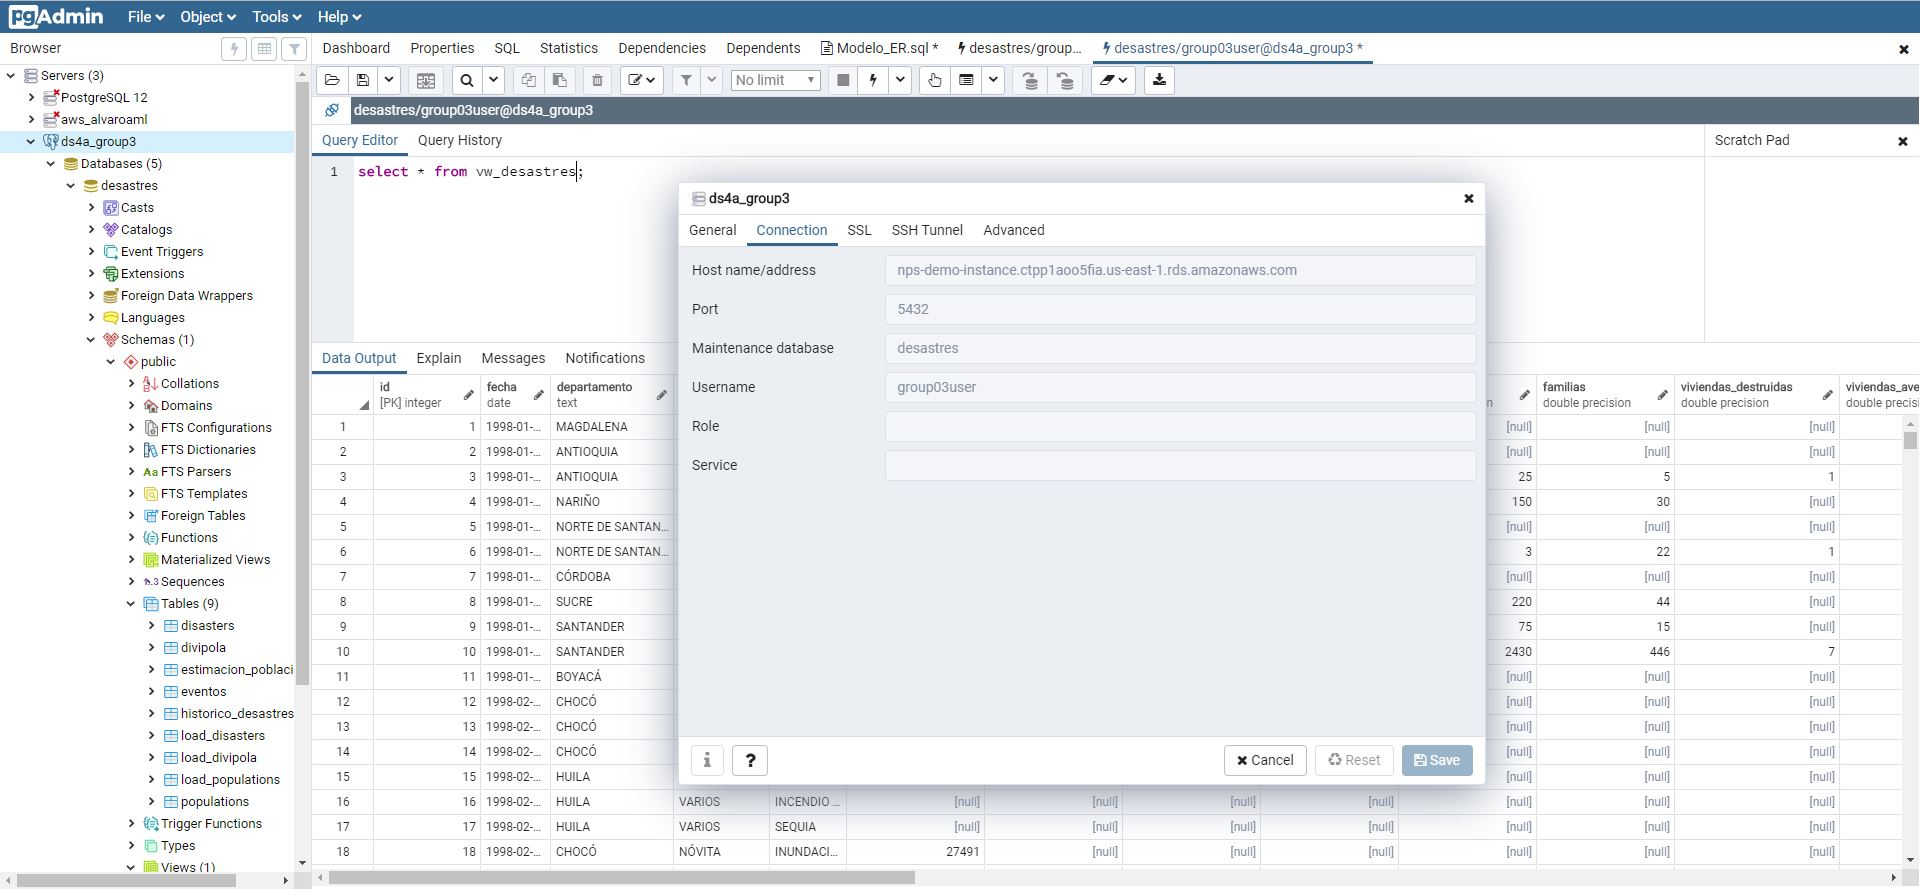
\includegraphics[width=0.95\textwidth]
{Desastres_AWS_Connection}}
\caption{AWS connection.}
\label{fig:awsConnection}
\end{figure}


Figure \ref{fig:databaseLoaded}  shows the database loaded to the AWS hosted database.

\begin{figure}[!htb]
\center{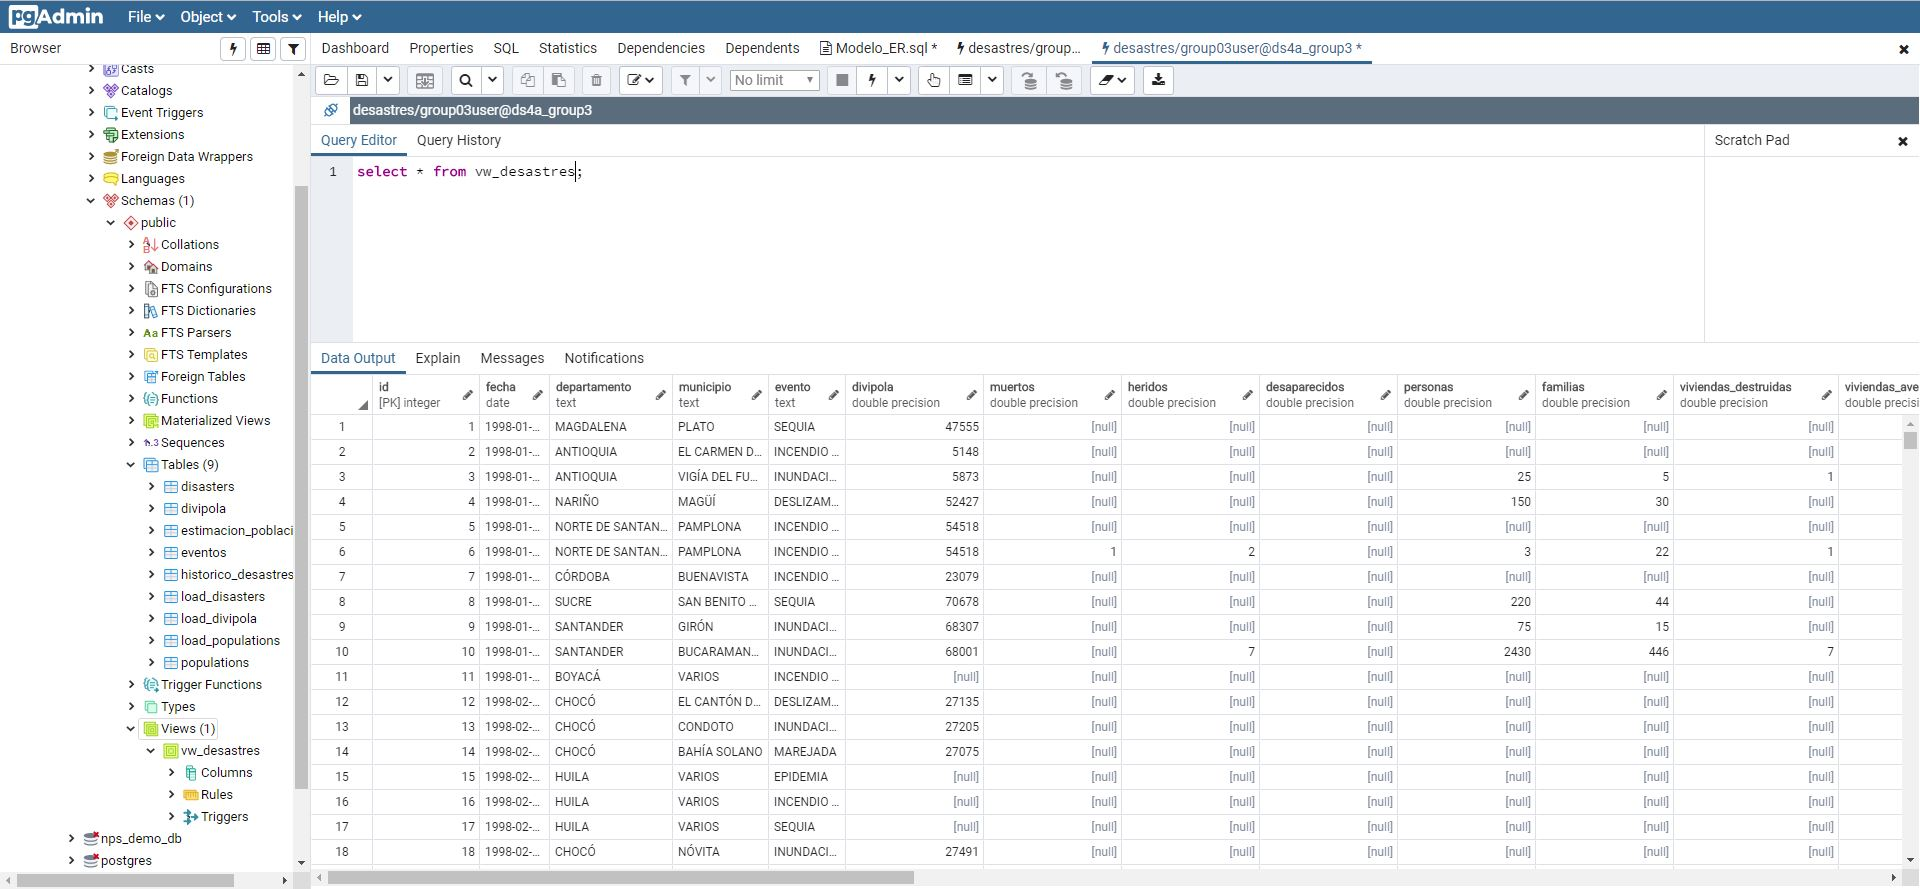
\includegraphics[width=0.95\textwidth]
{Desastres_data}}
\caption{Database loaded to AWS.}
\label{fig:databaseLoaded}
\end{figure}


The link between the front-end and the AWS-hosted databased was also stablished (see Figure \ref{fig:linkDASH_AWS}). 

\begin{figure}[!htb]
\center{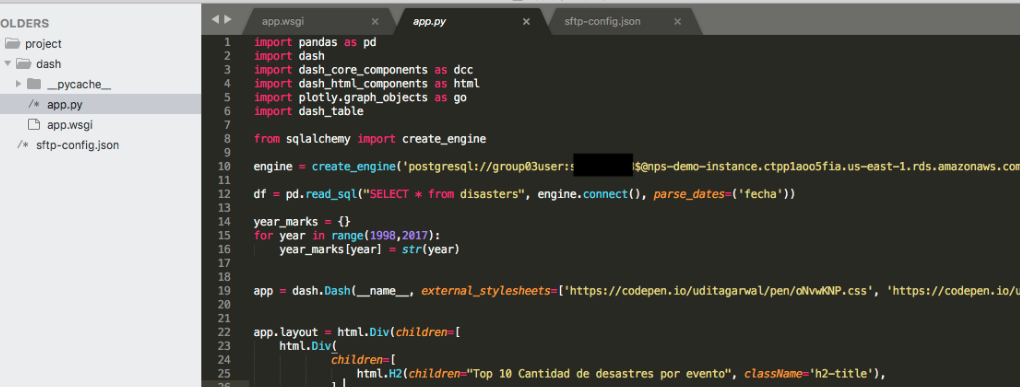
\includegraphics[width=0.95\textwidth]
{link_dash_aws}}
\caption{Link between DASH and AWS stablished}
\label{fig:linkDASH_AWS}
\end{figure}






\bibliographystyle{abbrv}
\bibliography{project}

\end{document}
This is never printed
